\documentclass{article}
\PassOptionsToPackage{numbers,sort&compress}{natbib}
\usepackage[preprint]{neurips_2025}
\usepackage[utf8]{inputenc}
\usepackage[T1]{fontenc}
\usepackage{amsmath,amssymb,booktabs,tabularx,array,graphicx,microtype}
\usepackage[hidelinks]{hyperref}
\usepackage{url}
\makeatletter
\renewcommand{\@noticestring}{ECE285: Deep Generative Models, UC San Diego. Fall 2026 mid-term report.}
\makeatother
\title{Conditional Generation of Lithium-Vacancy\\Configurations for Cathode Relithiation}
\author{Ricardo Silva Buarque \quad Beihao Gu \quad Varad Kottawar\\
University of California San Diego}
\newcommand{\KL}{D_{\mathrm{KL}}}
\newcommand{\E}{\mathbb E}
\begin{document}
\maketitle
\begin{abstract}
We study conditional generation of lithium-vacancy patterns in LiCoO$_2$, a
battery cathode material. Each example specifies which lithium sites are
occupied, and the generator is asked for new patterns at a given lithium
content and energy range. We compare conditional variational autoencoders
(CVAEs), autoregressive models and simple sampling baselines, measuring distinct
qualifying configurations per attempt. With energies evaluated by the pretrained
neural potential UMA, the spatial CVAE, its autoregressive control and mutation
achieve 62.20\%, 63.04\% and 58.37\% balanced yield. Neighbor information improves
yield, whereas increasing latent dimension improves reconstruction without a
consistent sampling benefit. Controlled interventions show that the energy
condition influences generation much more than the latent vector. Training on
energies after atomic relaxation also fails to improve the matched relaxed-energy
test. These comparisons support spatial conditional sampling without establishing
a latent-specific advantage, and show why useful latent learning needs
validation beyond reconstruction.
\end{abstract}

\section{Research question, motivation and related work}
A lithium-ion battery cathode stores and releases lithium during cycling.
Recycling can restore this material by replenishing missing lithium rather than
breaking it down into its constituent elements. Hydrothermal relithiation,
which uses heated water-based processing, has regenerated spent lithium cobalt
oxide, LiCoO$_2$ (LCO) \citep{shi2018}. At a fixed lithium content, there are many
ways to distribute the occupied and empty lithium sites. These arrangements can
have different energies because their neighboring atomic environments differ
\citep{vanderVen1998}. Finding useful arrangements is therefore a conditional
generation problem with a combinatorially large discrete output space.

Energy is a property of the atom types, positions and repeating simulation cell.
Density functional theory (DFT) calculates an approximate electronic structure
and serves as a reference for these energies and the forces on atoms, but is
expensive for large datasets. A machine-learned interatomic potential (MLIP) is
a model trained to approximate such calculations. It predicts energy from an
atomic structure; forces describe how that energy changes when atoms move.
Here, pretrained MLIPs provide inexpensive energy labels and score generated
samples. A \emph{single-point} evaluation leaves all positions fixed, whereas
\emph{geometry relaxation} repeatedly moves atoms using the predicted forces to
approach a local energy minimum. Generating a vacancy pattern alone does not
perform that minimization.

We ask: \textbf{can a CVAE generate new configurations in a requested energy
range more efficiently than uniform sampling and local mutation, and which
representations improve this yield?}

Wakamiya and Ishikawa
\citep{wakamiya2026} study a related problem for platinum/nickel catalyst
surfaces. Their convolutional CVAE learns grids specifying which element
occupies each site. It conditions on favorable classes of formation energy
(a stability measure) and oxygen-reduction overpotential (the extra voltage
needed to drive a catalytic reaction), then iteratively evaluates and retrains
on generated arrangements. Their evaluator already uses UMA, a universal MLIP
\citep{uma2025}. Our contribution is a controlled study of periodic vacancy
patterns: exact composition, symmetry-aware novelty, neighbor representations,
and a model without latent variables distinguish the causes of any sampling gain.

Targeting several energy ranges, including low-energy configurations, is useful
for assembling MLIP fine-tuning data. The potential energy surface maps atomic
arrangements to energy; covering diverse arrangements at different energies can
provide information beyond repeatedly sampling a few minima. Our energy classes
are intended to support that coverage. Whether the resulting data actually
improve a fine-tuned potential remains a separate validation question.

\section{Training data and structural representation}
\paragraph{What a configuration contains.}
We start from a repeating cell with 48 lithium, 48 cobalt and 96 oxygen atoms,
Li$_{48}$Co$_{48}$O$_{96}$. Its atomic arrangement is called \emph{O3}: one
particular layered structure in which lithium layers alternate with cobalt--oxygen
slabs. Periodic boundaries repeat the cell in all three directions, so a site
near one cell boundary can neighbor a site across the opposite boundary.
Removing selected lithium atoms creates a configuration. The 144 cobalt/oxygen
atoms, the remaining lithium coordinates and the cell stay fixed for the main
dataset; these examples are \emph{not} geometry-optimized vacancy structures.

An occupation mask $o\in\{0,1\}^{48}$ records $o_i=1$ for a present lithium atom
at site $i$ and $o_i=0$ for an empty site, or vacancy. The count
$n=\sum_i o_i\in\{12,24,36\}$ corresponds to lithium fractions
$x=n/48=0.25,0.50,0.75$; the structure contains $144+n$ atoms. UMA-S-1.2.1
with the \texttt{omat} setting supplies training energies. MACE-MH-1 with
\texttt{omat\_pbe} independently scores the same generated structures
\citep{uma2025,mace2022}. These are two pretrained energy models, not two
independent DFT reference datasets.

\paragraph{Periodicity and duplicate structures.}
An allowed translation, rotation or reflection of the periodic parent can turn one mask into
another without changing its physical arrangement. All masks related by the
192 retained parent-preserving site permutations form a \emph{symmetry orbit}.
We choose one canonical representative per orbit and group equivalent masks
before splitting the data. This prevents rotated or translated copies from
appearing as independent training and validation examples. The split contains
40,157 training, 4,967 validation and 5,123 test orbits. Only training examples
set model weights and energy thresholds; validation selects checkpoints. Test
examples are excluded from these decisions. For generation assessment, novelty
also excludes a fixed reference of 344,001 previously observed orbits, including
the training data.

\paragraph{Why neighboring environments matter.}
A binary vector tells the model which sites are occupied but does not explicitly
say which sites are physically close. Two masks with the same count can describe
clustered or dispersed vacancies. We therefore compare the ordered vector with
graph-based encoding, and give the decoder summaries of neighboring site states.
These are \emph{features}: numerical descriptions that make physically relevant
relationships accessible to the network. All features respect periodic neighbors.
The examples explore lithium ordering within one fixed O3 framework; other
layer stackings such as O2, three-dimensional spinel frameworks and atomic
rearrangements are absent. Especially at low lithium content, the starting
framework need not be stable. The model consequently learns a restricted
configuration distribution, not which crystal structure is chemically preferred.

\section{Conditional generation and evaluation}
\paragraph{What the condition requests.}
Energy labels are fitted separately at each lithium count. Training quantiles
$q_{20}$ and $q_{80}$ divide energy per present atom, $e$ in eV/atom, into
LOW ($e\le q_{20}$), MIDDLE ($q_{20}<e\le q_{80}$) and HIGH
($e>q_{80}$), with equal-energy ties kept together. The four-component condition
$c=(n/48,\operatorname{onehot}(b))$ combines lithium fraction with the requested
class $b$; for example, LOW has the three class entries $(1,0,0)$.
A low-energy request asks for a learned range, not an optimization gradient or
a guarantee of the lowest possible energy. Separate thresholds prevent the
composition-dependent energy baseline from determining the class. Each MLIP
uses its own training-derived thresholds when evaluating proposals.

\paragraph{How a CVAE generates a mask.}
The encoder sees the complete training mask and condition. It returns a Gaussian
$q_\phi(z\mid o,c)=\mathcal N(\mu_\phi,\operatorname{diag}\sigma_\phi^2)$
over a short latent vector $z\in\mathbb R^D$. The mean $\mu_\phi$ and variance
$\sigma_\phi^2$ are learned functions of the input. During training,
$z=\mu_\phi+\sigma_\phi\odot\epsilon$, with
$\epsilon\sim\mathcal N(0,I)$, allows gradients through the random sample.
During generation there is no input mask: $z$ is drawn from the fixed prior
$p(z)=\mathcal N(0,I)$, and the decoder constructs a new mask
\citep{kingma2014,sohn2015}.

A gated recurrent unit (GRU) with 64 hidden channels makes the 48 occupied/vacant
decisions in a fixed order. The probability factorization and training loss are
\begin{equation}
p_\theta(o\mid z,c)=\prod_{i=1}^{48}p_\theta(o_i\mid o_{<i},z,c,h_i),
\qquad
\mathcal L=-\E_{q_\phi}\log p_\theta(o\mid z,c)+\beta_t\KL(q_\phi\Vert p).
\label{eq:cvae}
\end{equation}
Here $\theta,\phi$ are decoder/encoder parameters, $o_{<i}$ contains the decisions
before site $i$, and $h_i$ summarizes their neighboring environments. The first
loss term rewards reconstruction of training masks. The Kullback--Leibler (KL)
term encourages the encoder distributions to resemble the prior from which we
will sample; $\beta_t$ controls its weight at update $t$. Both terms use natural
logarithms and are measured in nats per mask. Training supplies the true preceding
bits (teacher forcing); generation uses preceding sampled bits. To enforce the
requested count exactly, later decisions are forced vacant when no lithium
remains, or occupied when every remaining site is needed.

\paragraph{What the model comparisons isolate.}
The dense encoder uses 128 then 64 hidden units to process the ordered mask and
condition. The graph encoder instead represents atoms and candidate lithium
sites as nodes, retaining empty lithium sites so their locations are known.
Two width-32 message-passing layers exchange information over periodic neighbors
within 5~\AA, using six distance channels; pooled host and lithium-site features
produce the Gaussian parameters \citep{gilmer2017}.

The decoder has a different information constraint. Before deciding a site, it
can know which nearby sites are already occupied, already vacant, or not yet
assigned, but cannot see future target bits. The six-feature baseline summarizes
these three states using nearest-neighbor and exponentially distance-weighted
neighborhoods. The nine-feature alternative separates them into three distance
shells at 2.811, 4.869 and 4.912~\AA, including neighbors in adjacent layers.
This directly supplies local geometry while preserving causal generation.

\begin{table}[htbp]
\centering\small
\caption{Model comparisons. All listed CVAEs have $D=4$. AR denotes autoregressive
sampling without an encoder or latent vector.}
\label{tab:features}
\begin{tabularx}{\linewidth}{@{}l l X@{}}
\toprule Model & Encoder & Question tested\\
\midrule
A: graph CVAE & Graph Gaussian & Do latent variables help when spatial context is supplied?\\
B: spatial AR & None & Can the same spatial decoding rule work without a latent?\\
C: dense CVAE & Dense Gaussian & Does a different encoder improve generation with the same decoder?\\
D: scrambled AR & None & What happens when spatial associations are scrambled?\\
A-shell/B-shell & Graph/none & Does resolving three neighbor shells improve yield?\\
\bottomrule
\end{tabularx}
\end{table}

The AR control retains the decoder width, condition and neighbor features while
removing $z$. It still samples each decision randomly. The scrambled control
reassigns neighbors nonphysically while retaining overall weights and parameter
count; this also changes when information becomes available along the sequence,
so it does not isolate distance alone. Shell features add 576 GRU parameters,
and graph/dense encoders have different capacities. These comparisons are
informative but not all strictly capacity-matched. Fixed-order decoding also
means the full model is not permutation-equivariant; canonicalization handles
the retained parent symmetries.

\paragraph{Training and model selection.}
Each fit uses Adam, learning rate $10^{-3}$, batch size 512 and 4,000 updates.
The KL weight gradually rises to 0.1. Training class weights compensate for the
roughly 20/60/20 LOW/MIDDLE/HIGH imbalance; validation keeps the original example weights.
Checkpoints minimize validation reconstruction plus $0.1$KL, using fixed random
noise for comparable validation estimates. Model selection uses development
comparisons; the final sampling assessment does not select or modify models.

\paragraph{What counts as successful generation.}
Uniform sampling chooses exactly $n$ lithium sites at random. Mutation starts
from a training mask in the requested energy class and swaps one, two or three
occupied sites with the same number of vacancies, preserving composition.
These baselines test whether learning improves on random exploration and on
small edits to already useful examples.

Our primary score asks how many attempts produce a genuinely new arrangement
in the requested range. For replicate $s$, count $n$ and class $b$,
\begin{equation}
Y_{snb}=\frac{\#\{\text{distinct valid orbits absent from the reference and measured in class }b\}}
{\#\{\text{all attempted proposals at }(s,n,b)\}}.
\label{eq:yield}
\end{equation}
Generating one qualifying arrangement ten times earns one discovery, not ten;
repeats, invalid outputs and failed requests still consume attempts. We average
the nine count/class cells equally to obtain \emph{balanced yield}, then report
the mean and standard deviation (SD) across fitted-model or baseline-sampling
replicates. Each cell receives 128 attempts. The comparison includes 44,928
primary attempts and 4,992 separate latent probes. Duplicate physical queries
are evaluated only once, without removing their attempts from the denominator.

\section{Representation and hyperparameter results}
\begin{figure}[!htbp]
\centering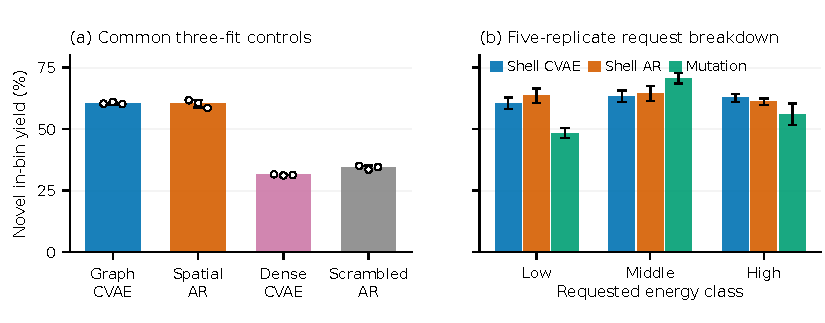
\includegraphics[width=\linewidth]{assets/featurization.pdf}
\caption{How representation changes useful sampling. Left: three matching fits per
control. Right: five fit/sampling replicates per energy request. Bars show means,
dots individual fits, and whiskers replicate SD. All energies use UMA. Mutation
is stronger for MIDDLE requests, so gains depend on the requested energy range.}
\label{fig:features}
\end{figure}

\paragraph{Neighbor features help both the CVAE and AR.}
With the same six decoder features, the graph CVAE and spatial AR have similar
yield: their paired difference over three matching fits is
$+0.20\pm1.49$ percentage points (pp). Dense encoding and scrambled spatial
associations give only $31.37\pm0.22\%$ and $34.38\pm0.80\%$
(Figure~\ref{fig:features}). Thus an encoder that can process the complete mask
is not sufficient; how the decoder receives neighboring information matters.

Separating three distance shells improves balanced UMA yield by
$1.96\pm0.32$~pp for the CVAE and $2.83\pm1.46$~pp for AR over five paired fits.
Table~\ref{tab:final} shows that both outperform uniform sampling and mutation
in balanced yield, with the shell AR giving the highest point estimate under
both teachers. The CVAE does not outperform this matched AR control
($-0.83\pm1.13$~pp under UMA). This does not prove that latent variables can
never help; no advantage is demonstrated at this data and training budget.
The gain over mutation is also not uniform: MIDDLE yield is 63.44\% for the
shell CVAE and 64.48\% for shell AR, versus 70.68\% for mutation.

\begin{table}[htbp]
\centering\small
\caption{Balanced novel in-request yield (\%, mean $\pm$ SD), five fit or sampling
replicates per row. MACE evaluates the same UMA-trained proposals using its own
training-derived energy classes. Agreement is a second-model check, not DFT validation.}
\label{tab:final}
\begin{tabular}{@{}lrr@{}}
\toprule Method & UMA & MACE\\
\midrule
Graph CVAE, six features & $60.24\pm0.53$ & $61.72\pm0.72$\\
AR, six features & $60.21\pm1.23$ & $62.03\pm0.76$\\
Graph CVAE, shell features & $62.20\pm0.56$ & $64.03\pm0.79$\\
AR, shell features & $63.04\pm1.47$ & $64.38\pm0.96$\\
Mutation & $58.37\pm1.08$ & $57.97\pm1.39$\\
Uniform fixed-count & $33.32\pm0.04$ & $33.32\pm0.04$\\
\bottomrule
\end{tabular}

\end{table}

\paragraph{More latent dimensions improve reconstruction, not reliably yield.}
A separate experiment varies $D\in\{4,8,16,32\}$ in a dense-encoder CVAE with the GRU decoder but no spatial
decoder features, with three fits per dimension and the same 4,000-update budget
(Figure~\ref{fig:dimension}). Validation reconstruction loss improves from
17.01 to 14.87 nats as $D$ grows, but useful yield ranges from 28.82\% to 32.64\%
without a monotonic trend. It stays near uniform sampling and below mutation
(59.72\%) within that experiment. Four dimensions provide an economical default,
but this is not evidence that four is optimal for the graph/shell architecture.
The dimension experiment uses a separate development proposal pool, so its
absolute yields should not be treated as a direct feature comparison with Table~\ref{tab:final}.

\begin{figure}[!htbp]
\centering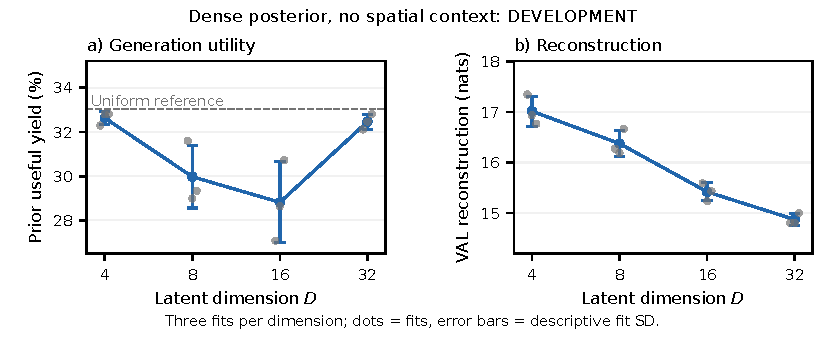
\includegraphics[width=\linewidth]{assets/latent_dimension.pdf}
\caption{Latent-dimension sensitivity for a dense encoder and GRU decoder without spatial
features. Three fits per dimension show better validation reconstruction with
larger $D$, but no consistent improvement in prior-sampling yield. Error bars
are fit SD. This is a finite sensitivity study, not demonstrated convergence.}
\label{fig:dimension}
\end{figure}

\paragraph{Class weighting and checkpoint choice.}
A dense-encoder/GRU experiment at $D=8$ asks whether rare energy classes need greater
training weight, and whether the validation criterion overemphasizes prior
matching. Table~\ref{tab:policy} compares equalized versus unadjusted training
class weights and two KL coefficients used to \emph{select checkpoints}. The
training loss still ends at $\beta=0.1$ in every case; changing checkpoint
selection is different from changing the training objective. The combination
of class balancing and selection coefficient 0.1 gives the best yield in this
comparison, showing that the validation objective can affect downstream
sampling even when the training objective is unchanged.

\begin{table}[htbp]
\centering\small
\caption{Dense-encoder/GRU $D=8$ development yield (\%, mean $\pm$ SD over three fits).
Columns change the validation selection criterion; rows change training weights.}
\label{tab:policy}
\begin{tabular}{@{}lrr@{}}
\toprule Training class weights & Selection KL weight 1 & Selection KL weight 0.1\\
\midrule
Unadjusted & $29.28\pm1.91$ & $30.44\pm0.66$\\
Class-balanced & $30.61\pm0.27$ & $32.12\pm0.63$\\
\bottomrule
\end{tabular}
\end{table}

A one-fit screen reducing the \emph{training} KL weight to 0.03 raises balanced
yield by 0.69~pp but lowers the separately tracked fixed-threshold low-energy
yield by 1.04~pp. This is not consistent evidence of improvement. Adding explicit
remaining-count features to spatial AR gives 61.40\% in three fits, below the
shell AR point estimate. Learning rate, batch size, widths, graph cutoff and
training duration were held fixed; no convergence claim is made for them.
The dimension study also changes parameter count with $D$, and further training
could change the comparison. The present evidence supports a compact model
with useful spatial context, not a globally optimized set of hyperparameters.

\section{Understanding the learned latent space}
The latent vector is intended to be a short code for an arrangement, but good
reconstruction does not establish that this code helps generate useful new
samples \citep{alemi2018}. Three questions must be separated: does the encoder
store information about a mask, does the decoder use $z$ when sampling, and
does the explicit energy request control the output? We examine all three.

\begin{figure}[!htbp]
\centering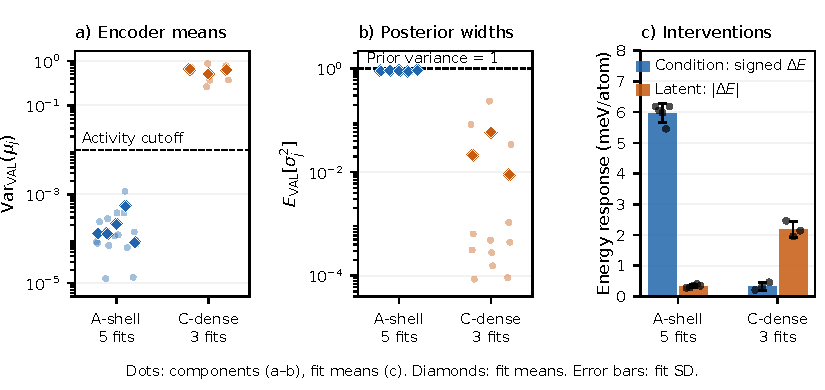
\includegraphics[width=\linewidth]{assets/latent_mechanism.pdf}
\caption{Encoder statistics and controlled sampling tests. A-shell uses five fits;
C-dense uses three and the six-feature decoder, so this is not an encoder-only
ablation. Components within a fit are not independent replicates. The 0.01
activity cutoff is heuristic. The last panel compares a signed LOW-to-HIGH
energy shift with an absolute change from varying $z$; these are distinct
observables. Diamonds and energy error bars show fit means and SD.}
\label{fig:latent}
\end{figure}

\paragraph{A wide distribution can still carry little information.}
For a useful encoder, different masks might produce distinguishable latent
means or variances. In the shell CVAE, mean posterior variances are
0.854--0.943, close to the unit variance of the prior, while posterior means
barely change across masks: their variances span
$1.26\times10^{-5}$--$1.16\times10^{-3}$. Using
$\operatorname{Var}(\mu_j)>0.01$ as a heuristic for an active coordinate gives
zero active coordinates in all five fits. Lowering that cutoff to 0.001 makes
one coordinate active in one fit. This supports near \emph{posterior collapse}:
the encoder distribution becomes almost independent of the input. It does
not mean that all samples have the same $z$, or that the latent distribution
has shrunk to one point; the distributions remain broad. A plausible mechanism
is that the decoder can predict from the condition and partial pattern without
needing $z$, while the KL term penalizes encoding extra information. This
interpretation is consistent with the no-latent control.

\paragraph{How much information can the code contain?}
The average validation KL is only 0.0072--0.0202 nats per mask (mean 0.0123).
To relate this to information, average encoder distributions over masks with
the same condition to obtain $q(z\mid c)$. Under the weighted empirical
validation distribution, the exact identity is
\begin{equation}
\underbrace{\E_{o,c}\KL(q_\phi(z\mid o,c)\Vert p(z))}_{\overline K}
=\underbrace{I_q(o;z\mid c)}_{\text{information about the mask}}
+\underbrace{\E_c\KL(q(z\mid c)\Vert p(z))}_{\text{averaged distribution's mismatch to the prior}}.
\label{eq:mi}
\end{equation}
Adding and subtracting $\log q(z\mid c)$ inside the KL separates the two terms.
Conditional mutual information $I_q(o;z\mid c)$ measures how much observing $z$
reveals about $o$ after the supplied condition is already known. Both right-hand
terms are nonnegative, so $I_q(o;z\mid c)\le\overline K$. Dividing the largest
observed KL by $\log 2$ gives an upper bound of approximately 0.030 bits per
mask. This bounds information under the stated empirical distribution; it is
not a direct mutual-information estimate, a population guarantee or a physical
configurational entropy. A large KL, conversely, need not mean useful information:
it can also reflect mismatch between the averaged encoder and the sampling prior.

\paragraph{Changing the condition has a much larger effect than changing the code.}
The CVAE's autoregressive decoder has two sources of randomness: the sampled latent
$z$ and the random numbers $U$ used for its occupied/vacant decisions. We can
write its output as $o=F_\theta(c,z,U)$. To isolate energy conditioning, we keep
$z,U$ fixed and change LOW to HIGH. The shell CVAE's mean UMA energy increases
by 5.97 meV/atom, where 1 meV is $10^{-3}$ eV. To isolate latent influence, we
instead keep $c,U$ fixed and resample only $z$. The mean absolute energy change
is just 0.335 meV/atom; on average 0.851 of the 48 occupation bits change, and
65.42\% of pairs remain in the same symmetry orbit. The energy request clearly
affects the output, while the latent contributes relatively little. Diversity
can still come from $U$, which also lets a no-latent AR generate different masks.

The dense CVAE illustrates the converse. Its KL is 12.52--13.32 nats and all
four coordinates are active. Changing $z$ alters 13.04 occupation bits on average,
yet changing LOW to HIGH shifts energy by only 0.331 meV/atom and its useful
yield is poor. An active code therefore does not guarantee effective conditional
sampling from the prior. The dimensions also have no assigned physical meaning;
their signs and order can change across fits. These tests describe what the
learned code does without assigning arbitrary axes to physical mechanisms.

\section{Relaxation targets and limitations}
\paragraph{Can the generator learn which masks become low-energy after atoms move?}
For a given mask, define $E_{\rm del}$ as the single-point energy at the fixed
starting coordinates and $E_{\rm end}$ as the energy reached after fixed-cell
atomic relaxation. The latter is a local endpoint, not a certified global
minimum. A paired dataset of 6,000 masks assigns 3,600 training, 1,200 validation
and 1,200 test roles before labeling. UMA relaxation uses FIRE, a force-based local optimizer,
and stops when the largest atomic force is below 0.05 eV/\AA, subject to
500-step and 120-second caps.
Eight interruptions are retained; usable fit data contain 3,594 training and
1,200 validation pairs.

We train three graph/shell CVAEs per energy target using matching initializations,
architecture and 4,000 updates. Only labels and training-derived class thresholds
differ. This directly tests whether knowing relaxed energies improves the choice
of masks; both models still output masks, and neither predicts relaxed coordinates.
Generated samples must actually be relaxed before evaluating $E_{\rm end}$.

At each lithium count, every generator is assessed against the same endpoint
bins fitted on the paired training data. Across 10,944 attempted proposals,
7,616 distinct physical queries all converge.
The six-feature graph CVAE, spatial AR and mutation reach endpoint LOW yields
of 65.63\%, 64.06\% and 53.82\%, respectively, in three replicates; CVAE minus
AR is $1.56\pm2.76$~pp. In the paired-data comparison, however, training on
$E_{\rm end}$ gives 60.42\% endpoint LOW yield versus 62.50\% when training on
$E_{\rm del}$ ($-2.08\pm2.76$~pp; no positive replicate). Balanced endpoint
yields are 58.74\% versus 59.14\%. Relaxed labels therefore do not improve this
controlled test. The large-corpus and paired-data models use different data and
neighbor features, so their absolute yields are not an architecture comparison.
Endpoint energies also require their own thresholds: relaxation lowers energies,
so applying unrelaxed thresholds would inflate apparent success.

\paragraph{What these results establish.}
Spatial conditional sampling produces new configurations in requested energy
ranges more efficiently than uniform masks, but a benefit specific to the
variational latent pathway remains unestablished. Replicate SD describes fit
variability, not a confidence interval; a few fits do not prove equivalence.
Symmetry-aware novelty establishes a different arrangement, not a distinct
relaxed minimum. The restriction to one O3 parent, three compositions and two
MLIPs leaves transfer to other sizes, materials and crystal frameworks untested.
The energy labels have not been established as DFT-accurate, and generated
frequencies are not equilibrium probabilities. Vacancy sampling also omits
atomic displacement, strain and magnetic variation, so energy-bin diversity
covers only part of the potential energy surface relevant to MLIP fine-tuning.
\clearpage
\bibliographystyle{unsrtnat}
\bibliography{references}
\end{document}
